\subsection{Differential-Mode \& Common-mode Gain}
The differential amplifier produced results that are clear and easily measurable when a small signal input is applied.
However, the differential-mode gain of the amplifier is observed to be a whole order of magnitude lower than the result from simulation.
Also, the common-mode gain of the amplifier is observed to be a whole order of magnirude higher than the result from simulation.
This may be partly due to high frequency attentuation since the circuit is operating at a relatively fast $1$\si{\mega\hertz} frequency. 
When the frequency of $v_{in}$ is changed to $1$\si{\kilo\hertz}, the output amplitudes increase.

\FloatBarrier

\begin{figure}[h!]
	\centering
	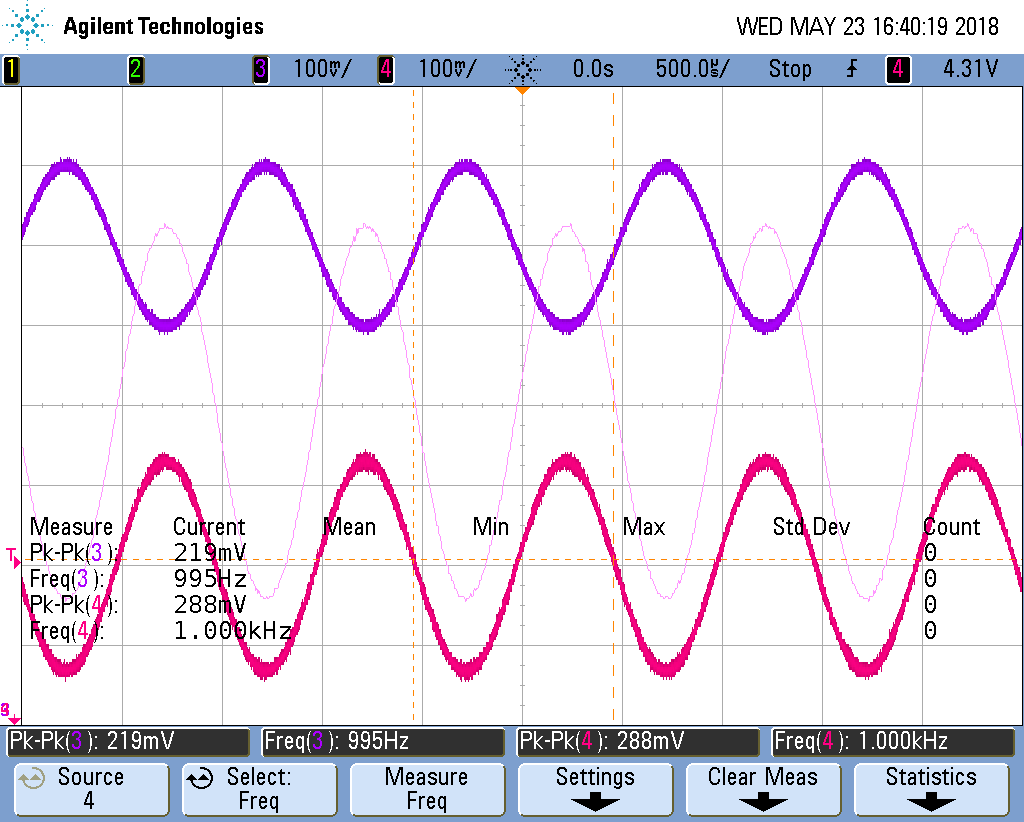
\includegraphics[scale=0.5]{./images/scope_2}
	\caption{$V_{out+}$ (4), $V_{out-}$ (3), and $V_{out+} - V_{out-}$ for $100$\si{\milli\volt} input at $1$\si{\kilo\hertz}}
	\label{fig:scope_2}
\end{figure}

\FloatBarrier

Also, it is observed that transistors M1A and M1B are mismatched as $V_{out+}$ and $V_{out-}$ vary by $60$\si{\milli\volt} and the drain currents on each side of the differential amplifier vary by $6$\si{\micro\ampere}.
Other inconsistancies may be due to slight variations in resistor values as well.
Overall, the differential amplifier exhibited behavior within the realm of expectation.
However, the performance of the amplifier is significantly worse than what simulation results would seem to indicate. \\



\subsection{Clamping \& Distortion}
When the input becomes too large, the output voltages are observed the clamp and distort because the transistors exit saturation.
When one transistor is near cutoff, the other is near triode, and vice-versa so that the differential mode output is large.
The voltage swing of $V_{out+}$, $V_{out-}$, and of $V_{out+} - V_{out-}$ is overall consistent with the simulated differential amplifier.
